% To documentclass. Αυτό τοποθετείτε στον cls κατάλογο και στο build του container κανονίζετε μόνο του!
\documentclass[
  11pt,
  singlespacing,
  liststotoc,
  toctotoc,
  headsepline
]{Assignments}

% Τα πακέτα του εγγράφου που χρησιμοποιούνται
% Πακέτα γλώσσας
\usepackage{alphabeta}
\usepackage{lmodern}

\usepackage{fontenc}
% \usepackage{xgreek}
% \usepackage{xunicode}
% \usepackage{xltxtra}

\usepackage[Greek,Latin]{ucharclasses}
\setTransitionsForGreek{\setlanguage{greek}}{\setlanguage{american}}

% Τα fonts του εγγράφου. Αυτά τοποθετούνται στον κατάλογο fonts
\setromanfont[Mapping=tex-text]{Linux Libertine}

\setmainfont{CMU Serif}
\setsansfont{CMU Sans Serif}
\newfontfamily{\greekfont}{CMU Serif}
\newfontfamily{\greekfontsf}{CMU Sans Serif}

\setmainfont{GFS Didot}

\usepackage[]{unicode-math}
\setmathfont{Latin Modern Math}

\usepackage[backend=bibtex,style=authoryear,natbib=true]{biblatex}

% Διαφορές βιβλιοθήκες με πολλαπλές χρήσης
\usepackage{graphicx} % Εμφάνιση γραφικών
\usepackage{booktabs} % Δημιουργία κεφαλαίων
\usepackage{enumerate} % Αρίθμηση
\usepackage{float}
\usepackage{minted} % Βιβλιοθήκη που διαβάζει κώδικα και τον χρωματίζει

% Βιβλιοθήκη που κάνει το reference των κεφαλαίων clickable. ΠΡΟΣΟΧΗ! μπαίνει πάντα τελευταίο.
\usepackage[hidelinks]{hyperref}

% Δημιουργία εξωφύλλου
\title{Self driving car} % Τίτλος εγγράφου
\author{I. Mastrogiannopoulos, S. Anagnostopoulos, P. Fiskilis, P. Zaritas} % Όνομα συγγραφέα/φοιτητή
\institute{University of West Attica \\ Department of Informatics and Computer Engineering} % Όνομα ιδρύματος και τμήματος φοιτητή
\class{Internet of Things} % Όνομα μαθήματος
\professor{Apostolos Anagnostopoulos} % Καθηγητής μαθήματος

% Αρχή του εγγράφου
\begin{document}

\includegraphics[width=25mm]{Figures/Logo} % Φωτογραφία
\maketitle % Δημιουργία τίτλου

% Abstract (μία μικρή σχετική περίληψη)
\begin{abstract}

\end{abstract}

\newpage % Νέα σελίδα
\tableofcontents % Πίνακας περιεχομένων
\listoffigures % Πίνακας εικόνων
\listoftables % Πίνακας πινάκων

\newpage
% \label{Chapter1}

% Το section αναφέρετε στο κεφάλαιο το οποίο θα δημιουργηθεί.
% Να παρατηρηθεί ότι αναγράφετε αυτόματα στον πίνακα περιεχομένων και είναι clickable.
\section{LaTeX tutorial}

% Το keyword \par αλλάζει παράγραφο
Μία παράγραφος \par
Δεύτερη παράγραφος. Τρίτη πρόταση

% Δημιουργία υπο-κεφαλαίου
\subsection{Υποκεφάλαιο}

% Χρήση κώδικα μέσα στο latex αρχείο
% Μέσα στο δεύτερο argument δέχεται την γλώσσα
\begin{minted}{tex}
\section{Chapter 1}
\subsection{Chapter 1.1}
\subsubsection{Chapter 1.1.1}
\end{minted}

Compile με: \mint{bash}{xelatex -shell-escape main.tex}

\subsubsection{Κώδικας python}
% Δεύτερο παράδειγμα
\begin{minted}{py}
print("Hello World!")
\end{minted}

\subsection{Εκφώνηση εργασίας}

% Το problem δημιουργεί ένα πλαίσιο γύρο από το κείμενο το οποίο μπορεί να
% χρησιμοποιηθεί για να αναφέρετε εκεί το ερώτημα που απαντιέται στο συγκεκριμένο σημείο
\begin{problem}
I, I will be king \par
And you, you will be queen \par
Though nothing will drive them away \par
We can beat them just for one day \par
We can be heroes just for one day \par
\par
And you, you can be mean \par
And I, I'll drink all the time \par
'Cause we're lovers, and that is a fact \par
Yes, we're lovers, and that is that \par
\end{problem}

Φοβερό τραγούδι από τον David Bowie! Το \href{https://www.youtube.com/watch?v=YLp2cW7ICCU}{Heroes} από τον ομότιτλο του album το 1977!

\subsection{Μαθηματικά}

Τύπος κατανομής Poisson.

% Έτσι δηλώνονται τα μαθηματικά στο latex. More on the internet...
\begin{equation}
  f_x(x) = e^-l * \frac{\lambda^x}{x!}, x = 0, 1, ...
\end{equation}

\subsection{Εικόνες}

% Έτσι δηλώνονται οι φωτογραφίες μέσα στο latex.
\begin{figure}[H] % Για να μείνει στο σημείο που τοποθετείτε, το [H] βοηθάει
  \centering % Για να μείνει στο κέντρο
  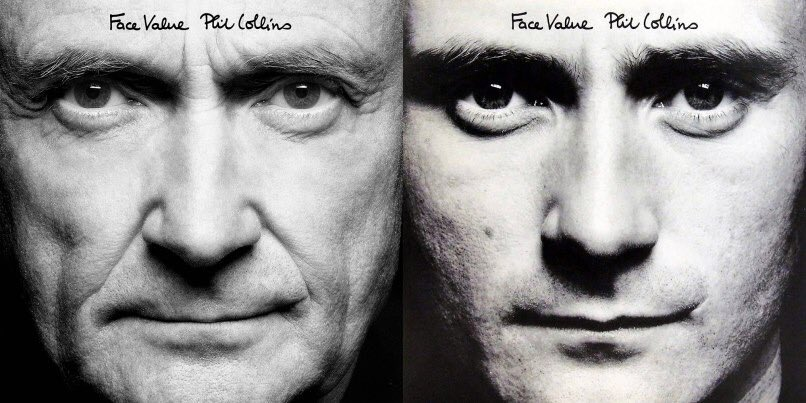
\includegraphics[width=100mm]{Figures/face_value} % Το width είναι το μέγεθος της εικόνας.
  \caption[Phil Collins - Face Value]{Δύο φωτογραφίες του διάσημου τραγουδιστή και drummer των Genesis, Phil Collins που τραβήχτηκαν σε δύο χρονικές περιόδους για το πρώτο του solo album, Face Value, 1981 και 2015}
  \label{fig:collins} % Με αυτό, θα μπορεί να χρησιμοποιηθεί αλλού στο έγγραφο για να γίνει δυναμική αναφορά της! Τρομερό!
\end{figure}

Επίσης πολύ καλό album του σχήματος~\ref{fig:collins}! Το πιο διάσημο τραγούδι του album είναι το \href{https://www.youtube.com/watch?v=IeDMnyQzS88}{In the Air Tonight}!

\subsection{Πίνακες}

Τυχαία αποτελέσματα στον πίνακα~\ref{tab:results_poisson_noise}. Ή μήπως όχι;

% Google this, it's more complicated than it looks
\begin{table}[H]
  \centering
  \begin{tabular}{| p{2cm} | p{7cm} | p{6.5cm} |}
  \hline
  \textbf{Φίλτρο} & \textbf{Αποτέλεσμα SSIM} & \textbf{Αποτέλεσμα Mean Square Error} \\
  \hline
  Γκαουσιανό φίλτρο & 0.7198557213172727 & 75.2685503882174 \\
  \hline
  Φίλτρο μέσης τιμής & 0.5889702706987753 & 99.21519127634552 \\
  \hline
  Φίλτρο διάμεσης τιμής & 0.42011072522698933 & 78.37677099175538 \\
  \hline
  \end{tabular}
  \caption{Τυχαία αποτελέσματα}
  \label{tab:results_poisson_noise}
\end{table}

\subsection{Λίστες}

Αγαπημένα συγκροτήματα!

\begin{itemize}
	\item Genesis
	\item Peter Gabriel
	\item The Beatles
	\item Pink Floyd
	\item Spock's Beard
	\item King Crimson
	\item David Bowie
\end{itemize}

Και αριθμημένα 10 αγαπημένα album από τον καθένα:

\begin{enumerate}
	\item The Lamb Lies Down on Broadway
	\item Peter Gabriel 3: Melt
	\item Abbey Road
	\item Wish You Were Here
	\item Snow
	\item Red
	\item Station to Station (or Low, or Ziggy Stardust)
\end{enumerate}

\section{ΠΕΡΙΣΣΟΤΕΡΑ ΣΤΟ GOOGLE}

Πήγε και τρεις και μίση το πρωί!
 % Include chapter1 από τον κατάλογο chapters. Μπορούν να προσδεθούν περισσότερα όσο μεγαλώνει το έγγραφο.
\end{document}
% Τέλος του εγγράφου